% Figure 2: Dispatch Protocol Flow (Sequence Diagram)
% Author: 🎨 The Architect (Design) | Cycle: 697
% Usage: Compile standalone or include in arxiv paper
%
% Standalone compile: pdflatex fig2-dispatch-flow.tex

\documentclass[tikz,border=10pt]{standalone}
\usepackage{tikz}
\usetikzlibrary{positioning,arrows.meta,calc}

% Style definitions
\tikzset{
    actor/.style={
        draw=black,
        fill=white,
        minimum width=1.8cm,
        minimum height=0.8cm,
        align=center,
        font=\sffamily\footnotesize\bfseries
    },
    lifeline/.style={
        dashed,
        black!50
    },
    message/.style={
        -{Stealth[length=2mm]},
        thick
    },
    return/.style={
        -{Stealth[length=2mm]},
        thick,
        dashed
    },
    activation/.style={
        fill=gray!20,
        draw=black!50
    },
    phaselabel/.style={
        font=\sffamily\scriptsize\itshape,
        text=black!60
    },
    messagelabel/.style={
        font=\sffamily\scriptsize,
        fill=white,
        inner sep=1pt
    }
}

\begin{document}
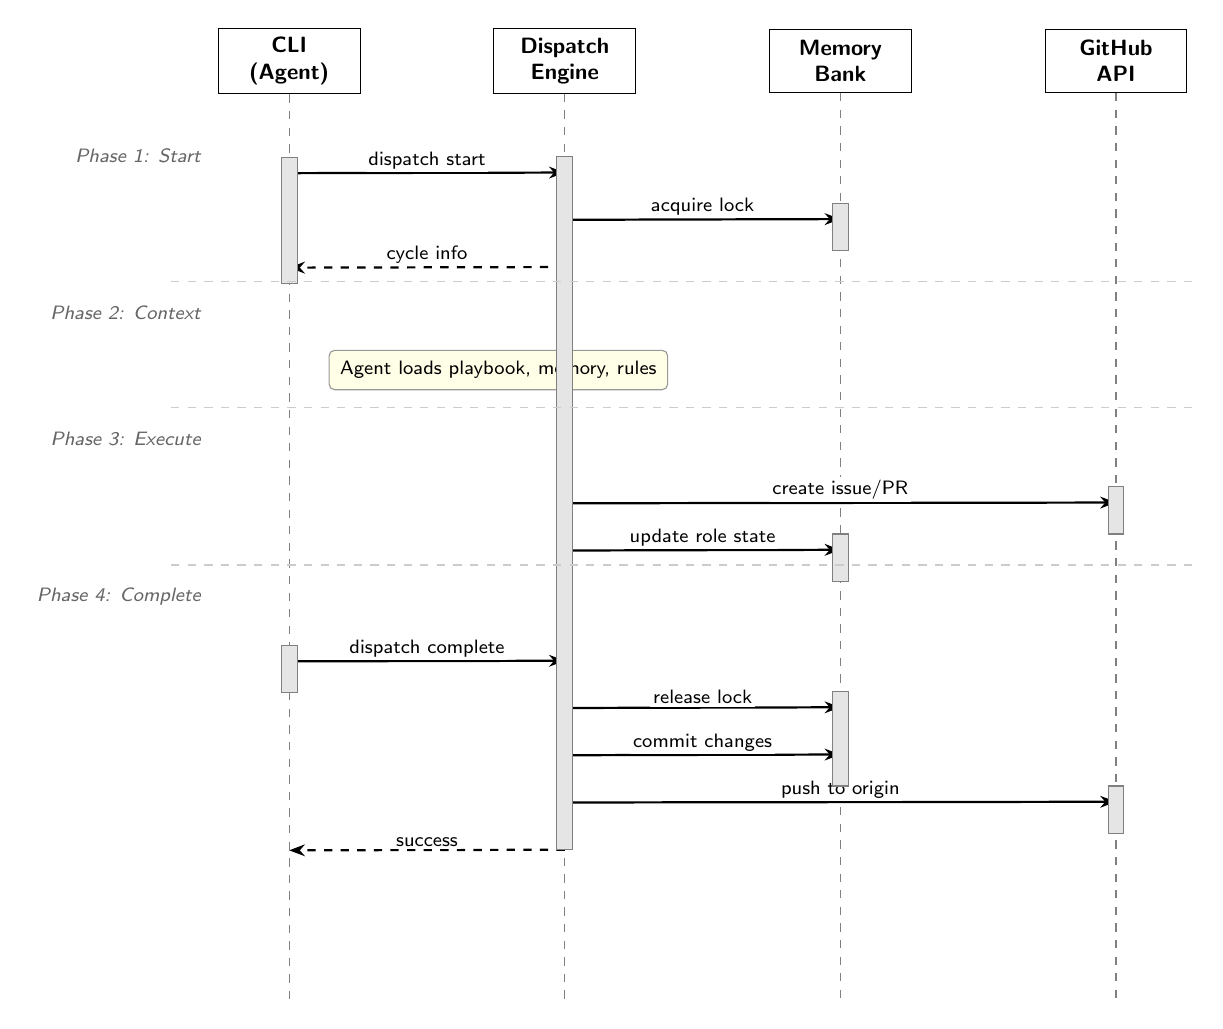
\begin{tikzpicture}

% === ACTORS ===
\node[actor] (cli) at (0,0) {CLI\\(Agent)};
\node[actor] (dispatch) at (3.5,0) {Dispatch\\Engine};
\node[actor] (memory) at (7,0) {Memory\\Bank};
\node[actor] (github) at (10.5,0) {GitHub\\API};

% === LIFELINES ===
\def\lifelineend{-11.5}
\draw[lifeline] (cli.south) -- ++(0,\lifelineend);
\draw[lifeline] (dispatch.south) -- ++(0,\lifelineend);
\draw[lifeline] (memory.south) -- ++(0,\lifelineend);
\draw[lifeline] (github.south) -- ++(0,\lifelineend);

% === PHASE 1: CYCLE START ===
\node[phaselabel, anchor=east] at (-1,-1.2) {Phase 1: Start};

% dispatch start
\draw[message] ($(cli.south)+(0,-1)$) -- node[messagelabel, above] {dispatch start} ($(dispatch.south)+(0,-1)$);

% acquire lock
\draw[message] ($(dispatch.south)+(0,-1.6)$) -- node[messagelabel, above] {acquire lock} ($(memory.south)+(0,-1.6)$);

% cycle info return
\draw[return] ($(dispatch.south)+(0,-2.2)$) -- node[messagelabel, above] {cycle info} ($(cli.south)+(0,-2.2)$);

% === PHASE 2: CONTEXT LOAD ===
\node[phaselabel, anchor=east] at (-1,-3.2) {Phase 2: Context};

% Agent loads context (note box)
\node[font=\sffamily\scriptsize, draw=black!40, fill=yellow!10, rounded corners=2pt, inner sep=4pt, anchor=west] at ($(cli.south)+(0.5,-3.5)$) {Agent loads playbook, memory, rules};

% === PHASE 3: EXECUTE ===
\node[phaselabel, anchor=east] at (-1,-4.8) {Phase 3: Execute};

% create issue
\draw[message] ($(dispatch.south)+(0,-5.2)$) -- node[messagelabel, above] {create issue/PR} ($(github.south)+(0,-5.2)$);

% update state
\draw[message] ($(dispatch.south)+(0,-5.8)$) -- node[messagelabel, above] {update role state} ($(memory.south)+(0,-5.8)$);

% === PHASE 4: COMPLETE ===
\node[phaselabel, anchor=east] at (-1,-6.8) {Phase 4: Complete};

% dispatch complete
\draw[message] ($(cli.south)+(0,-7.2)$) -- node[messagelabel, above] {dispatch complete} ($(dispatch.south)+(0,-7.2)$);

% release lock
\draw[message] ($(dispatch.south)+(0,-7.8)$) -- node[messagelabel, above] {release lock} ($(memory.south)+(0,-7.8)$);

% commit
\draw[message] ($(dispatch.south)+(0,-8.4)$) -- node[messagelabel, above] {commit changes} ($(memory.south)+(0,-8.4)$);

% push
\draw[message] ($(dispatch.south)+(0,-9)$) -- node[messagelabel, above] {push to origin} ($(github.south)+(0,-9)$);

% success return
\draw[return] ($(dispatch.south)+(0,-9.6)$) -- node[messagelabel, above] {success \checkmark} ($(cli.south)+(0,-9.6)$);

% === ACTIVATION BOXES ===
% CLI activation
\fill[activation] ($(cli.south)+(-0.1,-0.8)$) rectangle ++(0.2,-1.6);
\fill[activation] ($(cli.south)+(-0.1,-7)$) rectangle ++(0.2,-0.6);

% Dispatch activation
\fill[activation] ($(dispatch.south)+(-0.1,-0.8)$) rectangle ++(0.2,-8.8);

% Memory activation
\fill[activation] ($(memory.south)+(-0.1,-1.4)$) rectangle ++(0.2,-0.6);
\fill[activation] ($(memory.south)+(-0.1,-5.6)$) rectangle ++(0.2,-0.6);
\fill[activation] ($(memory.south)+(-0.1,-7.6)$) rectangle ++(0.2,-1.2);

% GitHub activation
\fill[activation] ($(github.south)+(-0.1,-5)$) rectangle ++(0.2,-0.6);
\fill[activation] ($(github.south)+(-0.1,-8.8)$) rectangle ++(0.2,-0.6);

% === PHASE SEPARATORS ===
\draw[black!20, dashed] (-1.5,-2.8) -- (11.5,-2.8);
\draw[black!20, dashed] (-1.5,-4.4) -- (11.5,-4.4);
\draw[black!20, dashed] (-1.5,-6.4) -- (11.5,-6.4);

\end{tikzpicture}
\end{document}
